%\documentclass[manuscript]{biometrika}
\documentclass[12pt]{article}

\usepackage{amsmath}
\usepackage{amssymb}
\usepackage{bm}
\usepackage{caption}
\usepackage{color}
\usepackage{enumerate}
\usepackage{graphicx}
\usepackage{natbib}
\usepackage{subcaption}
\usepackage{url}

%--------------------Initialize---------------------%
%\textheight= 9in  \textwidth = 6.5in \topmargin = -1.4cmg
%\oddsidemargin = -0.15in \evensidemargin = 0in
\bibpunct{(}{)}{;}{a}{,}{,}

\setlength{\textwidth}{6.5in} \setlength{\textheight}{9in}
\setlength{\topmargin}{-0.5in} \setlength{\oddsidemargin}{0.15in}
\setlength{\evensidemargin}{0.15in}

\renewcommand{\thefootnote}{\fnsymbol{footnote}}
\renewcommand{\baselinestretch}{1.75}

\newcommand{\pkg}[1]{{\normalfont\fontseries{b}\selectfont #1}}
\let\proglang=\textit
\let\code=\texttt

\newcommand{\ind}{\stackrel{\text{ind}}{\sim}}
\newcommand{\iid}{\stackrel{\text{iid}}{\sim}}
%\def \mone{\mbox{\boldmath$1$}}
%\def \mmu{\mbox{\boldmath$\mu$}}
%\def \mSigma{\mbox{\boldmath$\Sigma$}}
%\def \mI{\mbox{\boldmath$I$}}
%\def \mJ{\mbox{\boldmath$J$}}
%\def \mOmega{\mbox{\boldmath$\Omega$}}


%%% User-defined macros should be placed here, but keep them to a minimum.
\usepackage{graphicx}
\usepackage{color}


%% Here are the title, author names and addresses
\title{Fully Bayesian Benchmarking of Small Area Estimation Models}

\author{}
\date{}

\begin{document}

\maketitle

\begin{abstract}
Estimates for small areas defined by social, demographic, and geographic variables are increasingly important for official statistics. To overcome problems of small sample sizes, statisticians usually derive model-based estimates.  When aggregated, however, the model-based estimates typically do not agree with aggregate estimates obtained through more direct methods.  This lack of agreement between estimates can be problematic for users of small area estimates.  Benchmarking methods have been widely used to enforce agreement. Fully Bayesian benchmarking methods, in the sense of yielding full posterior distributions after benchmarking, can provide coherent measures of uncertainty for all quantities of interest, but research on them are limited.  We present a flexible fully Bayesian approach to benchmarking, in which benchmarks are incorporated into the likelihood.  The approach allows for a wide range of models and benchmarks.  We outline Markov chain Monte Carlo methods to generate samples from benchmarked posterior distributions.  We present two simulations, and an application to English and Welsh life expectancies.

{\it Keywords: Small Domain Estimation; Bayesian Hierarchical Model; Area-Level Model; Life Expectancy}
\end{abstract}

%\pagenumbering{arabic}

\section{Introduction}
  \label{sec:intro}

Small area estimation is the problem of obtaining estimates for many areas or domains defined by social, demographic and geographic variables where the number of observations in an area can be small. It has many practical applications, from monitoring unemployment to the targeting of anti-poverty programs \citep{pfeffermann2013new,rao2015small}, and is increasingly important for official statistics.  In the United States, for instance, county-level estimates from the Small Area Income and Poverty Estimates (SAIPE) program are used to allocate federal funding \citep{census2013saipe}.  In areas where the number of observations is small, `direct' methods, such as estimating rates by dividing the number of events in the area by the population at risk, perform poorly.  Small area estimation models compensate for small sample sizes by exploiting additional information, such as covariate data or values from similar areas.

Because of their practical importance, small area estimates often receive extensive public scrutiny.   This scrutiny typically includes a consistency check: estimates for small areas should agree with aggregate estimates for large areas, which are generally obtained using direct methods.  Model-based estimates of the number of poor people in each county, for instance, should add up to direct estimates of the number of poor people in the state.  Minor discrepancies may be tolerated, but major discrepancies undermine the credibility of the estimates.  Moreover, if estimates are used to allocate funding, discrepancies create grounds for dispute.  Many statistical offices and funding bodies accordingly have a ``one-figure'' policy, whereby estimates in different tables describing the same phenomenon must all agree with each other \citep[][p. 232]{dewaal2016obtaining}.  The US Census Bureau, for instance, adjusts county-level small area estimates to agree with state-level ones as part of the SAIPE program \citep{census2013saipe}.  Within the field of small area estimation, the aggregate estimates are referred to as benchmarks, and techniques for forcing small area estimates to agree with the benchmarks are known as benchmarking \citep{pfeffermann2013new}.

Many existing methods for benchmarking treat benchmarks as a type of constraint. The methods differ, however, in the way that the constraints are interpreted, and in the way that the constraints are incorporated into the estimation procedures.  Some methods follow a two-step procedure: first estimating the small area models, and then modifying the resulting point estimators to satisfy the benchmarking constraints \citep{you2004benchmarking,datta2011bayesian,berg2009spree,berg2012benchmarked,fabrizi2012constrained,steorts2013estimation,fabrizi2014mapping,ghosh2015benchmarked}.
Some methods treat benchmarks as constraints on the small area parameters and estimate the small area models under these constraints  \citep{pfeffermann1991some,pfeffermann2006small,fabrizi2012constrained,pfeffermann2014single}.  Some methods estimate the small area models under benchmarking constraints on the point estimators \citep{wang2008small,bell2013benchmarking}.  Some methods estimate the small area models or their augmented versions in such a way that the point estimators are self-benchmarked, i.e., the benchmarking constraints on the point estimators are automatically satisfied \citep[][Sections 4 and 5]{you2002pseudo,you2003pseudo,wang2008small,you2013performance,bell2013benchmarking}.

Most methods, including all of the ones cited above, focus on obtaining point estimates of small area parameters and associated uncertainty measures.  Some Bayesian benchmarking methods, however, provide probability distributions for small area parameters \citep{toto2010bayesian,nandram2011bayesian,nandram2011constraint,vesper2013three}.  These methods are fully Bayesian in the sense that they yield a full posterior distribution for all unknown quantities after benchmarking.  On this definition of fully Bayesian benchmarking, methods such as those of \citet{you2004benchmarking} and \citet{datta2011bayesian}, which derive posterior distributions without benchmarking but provide point estimators after benchmarking, are not fully Bayesian. The advantage of having a full posterior distribution is that it automatically  provides measures of uncertainty for all model parameters, small area parameters, and derived quantities.  For instance, it is easy to derive a full posterior distribution for the ranks of the small areas from richest to poorest, and to assess the uncertainty of these ranks.

In this paper, we present an approach to fully Bayesian benchmarking that can be applied to a wide range of small area models. We treat benchmarks as estimates for underlying aggregate parameters.  To measure agreement with the benchmarks, we specify a probability distribution for the benchmarks conditional on the aggregate parameters. We revise the likelihood function by multiplying the original likelihood function by the probability distribution for the benchmarks.  Multiplying the revised likelihood function by the prior distribution then yields the benchmarked posterior distribution.

In the main body of the paper, we focus on `area-level' models, as opposed to `unit-level' models \citep{rao2015small}.  Area-level models relate small area direct estimators to area-specific covariates.  The Fay-Herriot model \citep{fay1979estimates}, for instance, is a popular area-level model used for the estimation of small area means. Unit-level models relate the unit values of an outcome variable to unit-specific covariates.  The World Bank or ELL method \citep{elbers2003micro}, for instance, is a widely used method for estimating small area poverty indicators, in which a unit-level model is fitted using survey data, and then applied to census data to obtain values of the outcome for all units.  In Section 4 of the Supplemental data we discuss how our methods could be extended to unit-level models.

We implement our approach using Markov chain Monte Carlo (MCMC) methods.  The methods are designed to work with complicated models that would be difficult to benchmark using previous fully Bayesian benchmarking approaches.

Our approach accommodates multiple benchmarks, and benchmarks that are nonlinearly related to small-area quantities.  There is little previous research on nonlinear benchmarks: exceptions are \citet{datta2011bayesian} and \citet{fabrizi2012constrained}, who benchmark the variability of the point estimators after model estimation, which can be considered as special cases of nonlinear benchmarking.  In our application section, we estimate age-specific mortality rates benchmarked to life expectancies, which are nonlinearly related to the age-specific rates.

 Our approach also allows control over the degree of agreement between model-based estimates and benchmarks. In some applications, users require exact agreement between small areas estimates and benchmarks, while in others, they may tolerate minor discrepancies.  We refer to methods that achieve complete agreement as exact benchmarking, and methods that allow discrepancies as inexact benchmarking.  Almost all previous methods have implemented exact benchmarking.  Exceptions include \citet[][Section 2]{bell2013benchmarking}, \citet{nandram2011constraint}, and \citet{vesper2013three}.

The rest of the paper is organized as follows.  Section 2 describes our approach, including an outline of the associated MCMC methods.  Section 3 compares our approach with previous approaches.  Section 4 uses two simulation studies to illustrate the effect of benchmarking on the performance of small area models.  Section 5 applies our methods to the problem of estimating district-level life expectancy in England and Wales.  Section 6 summarizes the advantages of our methods.

\section{A Fully Bayesian Approach to Benchmarking}
  \label{sec:bayesian_interpretation}

\subsection{Conceptual Framework}
  \label{sec:problem}

We start with a standard setup for the fully Bayesian estimation of area-level models. The aim is to estimate area-level parameters $\bm{\gamma} = \{\gamma_1, \dots, \gamma_n\}^{\top}$, such as means, rates, or probabilities, on the $n$ areas defined by a multiway classification constructed from variables such as age, sex, and region.  The data are area-level observations $\bm{y}=\{y_1,\cdots,y_n\}$.  In a hierarchical Bayesian model, the likelihood is $p(\bm{y}\mid\bm{\gamma})$, the prior distribution is $p(\bm{\phi}) p(\bm{\gamma} | \bm{\phi})$, where $\bm{\phi}$ is a vector of hyperparameters, and the posterior distribution is
\begin{equation}
  p(\bm{\gamma}, \bm{\phi} |\bm{y})\propto p(\bm{\phi}) p(\bm{\gamma} | \bm{\phi}) p(\bm{y} | \bm{\gamma}). \label{eq:unbenchmarked_posterior}
\end{equation}
The prior may itself have a complicated hierarchical structure. Throughout the paper, we use Roman letters to denote data, and use Greek letters to denote parameters.

We extend this setup to incorporate benchmarking.  The statistician carrying out the small area estimation is provided with a set of benchmarks $\bm{m} = \{m_1, \dots, m_d\}^{\top}$, with $d$ much less than $n$. The benchmarks are pre-existing summary statistics at a more aggregate level than $\bm{y}$.   If $\bm{y}$ is numbers of people in the labor force disaggregated by age, sex, and education level, for example, then $\bm{m}$ might be estimates of labor force participation rates disaggregated only by sex.  If $\bm{y}$ is death counts disaggregated by age, sex and region, then $\bm{m}$ might be estimates of life expectancy by sex and region.  The statistician is required to make estimates of the area-level parameters $\bm{\gamma}$ agree with the benchmarks $\bm{m}$.

The benchmarks could be calculated from $\bm{y}$, or from other data sources.  Within the small area estimation literature, benchmarking where $\bm{m}$ is calculated from $\bm{y}$ itself is known as internal benchmarking, and benchmarking where $\bm{m}$ is calculated from other sources is known as external benchmarking \citep[e.g.][]{bell2013benchmarking}.

Decisions on whether to benchmark, on which statistics to benchmark to, on whether to use internal or external benchmarking, and on the degree of agreement required between small area estimates and benchmarks, are typically determined by the institutional setting and the specifics of the application. Statistical agencies often have a policy of using direct methods for aggregate measures where sample sizes are large, and using model-based methods to disaggregate further, with the requirement that model-based estimates agree with aggregate ones \citep{little2012calibrated}.  In other words, statistical agencies require statisticians to perform internal benchmarking.

If the small area estimates will be used to allocate funding, then exact benchmarking may be required, to avoid surpluses or shortfalls. In contrast, if the main users of small area estimates are researchers and policy analysts, then some discrepancies between small area estimates and aggregates estimates may be acceptable.

We distinguish between the benchmarks and the underlying parameters that they estimate. Let $\bm{\psi} = \{\psi_1, \dots, \psi_d\}^{\top}$ denote the parameters that the benchmarks $\bm{m}$ estimate. Vector $\bm{\psi}$ is derived from $\bm{\gamma}$ through a deterministic benchmarking function $\bm{\psi}=\bm{f}(\bm{\gamma})$, which consists of $d$ components $\psi_j=f_j(\bm{\gamma})$, $j=1,\dots,d$. For each benchmarking parameter $\psi_j$, let $\delta_j$ denote the set of areas $i$ such that $\gamma_i$ contributes to $\psi_j$.  We require that the $\delta_j$ do not overlap, in that each area $i$ belongs to at most one $\delta_j$. This restriction is commonly used in applications of benchmarking.

The components of the benchmarking function are typically linear, so that
\begin{equation}
   \psi_j = \sum_{i=1}^n b_{ij} \gamma_i, \quad i=1,\dots, n, \, j=1,\dots,d, \label{eq:benchmarking_constraint}
\end{equation}
where the $b_{ij}$ are known constants and $b_{ij}=0$ for $i\notin \delta_j$.  Equivalently, $\bm{\psi} = \bm{B}^{\top} \bm{\gamma}$ where $\bm{B}$ is a $n\times d$ matrix of $b_{ij}$. For example, if $\bm{\gamma}$ is labor force participation rates by age, sex and education level, and $\bm{\psi}$ is labor force participation rates by sex, then $\delta_j$ consists of all areas associated with sex $j$, and $b_{ij}=w_i/\sum_{i'\in \delta_j}w_{i'}$, where $w_i$ is the population count for area $i$.  However, the components of the benchmarking function may also be nonlinear.  For example, if $\bm{\gamma}$ is mortality rates by age, sex and region, and $\bm{\psi}$ is life expectancy by sex and region, then $\delta_j$ consists of all areas associated with each combination $j$ of sex and region, and $f_j$ is a nonlinear deterministic function of $\{\gamma_{i}:\ i\in\delta_j\}$ \citep[][ch. 3]{preston2001demography}.

To measure agreement with the benchmarks, we specify a probability distribution for the benchmarks conditional on the aggregate parameters, $p^{[\bm{m}|\bm{\psi}]}(\bm{m}|\bm{\psi})=p^{[\bm{m}|\bm{\psi}]}(\bm{m}|\bm{f}(\bm{\gamma}))$.  We then multiply the original likelihood $p(\bm{y}|\bm{\gamma})$ by this distribution. The modified likelihood $p(\bm{y}|\bm{\gamma})p^{[\bm{m}|\bm{\psi}]}(\bm{m}|\bm{f}(\bm{\gamma}))$ is a compromise between the original likelihood and the requirement to agree with the benchmarks.  The component $p^{[\bm{m}|\bm{\psi}]}(\bm{m}|\bm{f}(\bm{\gamma}))$ pulls the original likelihood towards the benchmarks.  For values of $\bm{\gamma}$ yielding larger (smaller) values for $p^{[\bm{m}|\bm{\psi}]}(\bm{m}|\bm{f}(\bm{\gamma}))$, the original likelihood is inflated (deflated).

In the special case of external benchmarking where $\bm{m}$ comes from completely separate data sources from $\bm{y}$ and where $p^{[\bm{m}|\bm{\psi}]}$ describes the sampling distribution of $\bm{m}$ given $\bm{\psi}$, the revised likelihood gives the joint distribution of $\bm{y}$ and $\bm{m}$ given the parameters $\bm{\gamma}$.  But in general $p^{[\bm{m}|\bm{\psi}]}$ cannot be interpreted as a standard component of the likelihood, but rather as a device for enforcing the extra requirement to agree with the benchmarks.

 With the revised likelihood, the benchmarked posterior distribution is given by
\begin{equation}
  p(\bm{\gamma},\bm{\phi}|\bm{y},\bm{m})\propto p(\bm{\phi}) p(\bm{\gamma} | \bm{\phi}) p(\bm{y} | \bm{\gamma})p^{[\bm{m}|\bm{\psi}]}(\bm{m}|f(\bm{\gamma})).\label{eq:benchmarked-posterior}
\end{equation}

\subsection{Exact Benchmarking}\label{sec:exact}

Under exact benchmarking, model-based estimates are required to agree perfectly with the benchmarks.  We interpret perfect agreement to mean that
\begin{equation}
  p^{[\bm{m}|\bm{\psi}]}(\bm{m} | \bm{\psi}) = \begin{cases} 1 & \text{ if } \bm{m} = \bm{\psi}\text{;} \\ 0 & \text{ otherwise.} \end{cases}
  \label{eq:model_exact_benchmarking}
\end{equation}


This interpretation of exact benchmarking is effectively the same as the one adopted by \citet{pfeffermann1991some}, \citet{pfeffermann2006small}, \citet{fabrizi2012constrained}, and \cite{pfeffermann2014single}, all of whom take frequentist approaches, and \citet{nandram2011constraint}, who take a fully Bayesian approach.  These methods all treat the benchmarks as constraints on the small area parameters.

When \eqref{eq:model_exact_benchmarking} is plugged into \eqref{eq:benchmarked-posterior}, the benchmarked posterior distribution becomes a singular distribution concentrated on the region $\{(\bm{\gamma},\bm{\phi}): \bm{f}(\bm{\gamma})=\bm{m}\}$. Every $\bm{\gamma}$ in the posterior distribution satisfies the restriction $\bm{f}(\bm{\gamma}) = \bm{m}$. Therefore, any point estimate $\hat{\bm{\gamma}}$ of $\bm{\gamma}$, such as the posterior mean or posterior median, satisfies $\bm{f}(\hat{\bm{\gamma}})=\bm{m}$. We show how samples can be generated from the singular posterior distribution in Section~\ref{sec:general_algorithm}.

\subsection{Inexact Benchmarking}\label{sec:inexact}

Under inexact benchmarking, $p^{[\bm{m}|\bm{\psi}]}$ is a non-degenerate distribution. The statistician can define $p^{[\bm{m}|\bm{\psi}]}$ so that it operationalizes the definition required by the particular institutional setting.  For example, if it is required that most discrepancies are smaller than a given tolerance $a$, such that $\text{Pr}(|m_j-\psi_j|<a|\psi_j)\geq q$ for $j=1,\cdots,d$, then it may be appropriate to specify $p^{[\bm{m}|\bm{\psi}]}$ as
\begin{equation}
m_j\ind \text{N}\left(\psi_j,\left(\frac{a}{z_{(1-q)/2}}\right)^2\right),
\end{equation}
where $\ind$ indicates independent distributions, and $z_{(1-q)/2}$ is the upper $(1-q)/2$ quantile of a standard normal distribution.

In some applications, the sampling distribution of $\bm{m}$ given $\bm{\psi}$, $p^{[\bm{m}|\bm{\psi}]}_{\text{sample}}$, is known, and it may be appropriate to incorporate the sampling distribution into the measure of agreement.  The measure can be customized by including a tuning parameter $\lambda$, with smaller values of $\lambda$ enforcing greater agreement.  We illustrate with two examples.

In the first example, the data $\bm{y}$ are obtained from a survey, and the benchmarks $\bm{m}$ are direct estimates calculated from $\bm{y}$, with standard errors $\bm{s}$.  If the survey was implemented well, then $\bm{m}$ should be unbiased for $\bm{\psi}$, and $\bm{s}$ should be approximately correct. If each $m_j$ is derived from a large number of observations, then we can assume that, conditional on the $\psi_j$, each $m_j$ is independently normally distributed with mean $\psi_j$ and standard deviation $s_j$.  The sampling distribution $p^{[\bm{m}|\bm{\psi}]}_{\text{sample}}$ is given by
\begin{equation}
p^{[\bm{m}|\bm{\psi}]}_{\text{sample}}(\bm{m}|\bm{\psi})\propto\text{exp}\left( - \sum_{j=1}^d \frac{ ( m_j-\psi_j)^2}{ 2 s_j^2} \right). \label{eq:dist-normal-sam}
\end{equation}
Incorporating a tuning parameter $0 < \lambda \leq 1$ into \eqref{eq:dist-normal-sam} yields
\begin{equation}
p^{[\bm{m}|\bm{\psi}]}(\bm{m}|\bm{\psi})\propto\text{exp}\left( - \sum_{j=1}^d \frac{ ( m_j-\psi_j)^2}{ 2 \lambda s_j^2} \right). \label{eq:dist-normal}
\end{equation}
When $\lambda\rightarrow 0$, \eqref{eq:dist-normal} converges to \eqref{eq:model_exact_benchmarking}.  Hence exact benchmarking is a limiting case of inexact benchmarking.

In the second example, the data are counts of events that follow Poisson distributions.  We have $y_i\sim \text{Poisson}(w_i\gamma_i)$, where $w_i$ is the known exposure for area $i$.  Let $v_j=\sum_{i\in\delta_j}w_i$ denote the total exposure associated with $\delta_j$. Then $\psi_j=\sum_{i\in\delta_j}w_i\gamma_i/v_j$, and its estimate is $m_j=\sum_{i\in\delta_j}y_i/v_j$, where $\sum_{i\in\delta_j}y_i
\sim \text{Poisson}(\sum_{i\in\delta_j}w_i\gamma_i)\sim\text{Poisson}(v_j\psi_j)$. The sampling distribution $p^{[\bm{m}|\bm{\psi}]}_{\text{sample}}$ is given by
\begin{equation}
p^{[\bm{m}|\bm{\psi}]}_{\text{sample}}(\bm{m}|\bm{\psi})\propto \prod_{j=1}^d \text{Poisson}(v_j m_j |  v_j\psi_j). \label{eq:dist-poisson-sam}
\end{equation}
Incorporating a tuning parameter $0 < \lambda \leq 1$ into \eqref{eq:dist-poisson-sam} yields
\begin{equation}
p^{[\bm{m}|\bm{\psi}]}(\bm{m}|\bm{\psi})\propto \prod_{j=1}^d \text{Poisson}(\lambda v_j m_j|  \lambda v_j\psi_j), \label{eq:dist-poisson}
\end{equation}
with convergence to exact benchmaking as $\lambda \rightarrow 0$.

In the above examples of $p^{[\bm{m}|\bm{\psi}]}$, we have assumed conditional independence of $m_j$'s given the underlying parameters $\psi_j$'s, and used simple models for $p(m_j|\psi_j)$.  This is similar to assuming conditional independence of $y_i$'s given $\gamma_i$'s and using simple models for $p(y_i|\gamma_i)$.  Unconditionally, the $m_j$'s can have complicated correlations, such as correlations between neighbouring time points or age groups. Such correlations are captured by the prior model on the underlying benchmarking parameters $\bm{\psi}$, which is implied by the prior model on $\bm{\gamma}$, $p(\bm{\phi})p(\bm{\gamma}|\bm{\phi})$, and the equality $\bm{\psi}=\bm{f}(\bm{\gamma})$.  The prior model on $\bm{\gamma}$ typically uses a complicated hierarchical structure to model relationship between the underlying parameters, such as similarities between neighbouring time points or age groups.

\subsection{An Illustrative Analytical Example}
  \label{sec:anal}

To illustrate the benchmarked posterior distribution, we present an example in which the distribution can be derived in closed form. The data $\bm{y} = \{y_1, \dots, y_n\}$ are generated and modelled using
\begin{align}
  y_i &\ind \text{N}(\gamma_i,\sigma^2) \label{eq:anal_fitted_model_lik} \\
  \gamma_i & \ind \text{N}(\mu_0,\tau^2) \label{eq:anal_fitted_model_pr},
\end{align}
where $\sigma^2$ and $\tau^2$ are known.  There is a single benchmark $m = \bar{y}\equiv \sum_{i=1}^n y_i / n$ estimating benchmarking parameter $\psi = \sum_{i=1}^n \gamma_i / n$. Under exact benchmarking, $p^{[m|\psi]}$ is given by \eqref{eq:model_exact_benchmarking}.  Under inexact benchmarking, the sampling distribution $p^{[m|\psi]}_{\text{sample}}$ is given by
\begin{equation}
p^{[m|\psi]}_{\text{sample}}(m|\psi) \sim \text{N}(\psi, \sigma^2/n).\label{eq:anal-dist-samp}
\end{equation}
We incorporate a tuning parameter $\lambda$ into \eqref{eq:anal-dist-samp} and arrive at
\begin{equation}
p^{[m|\psi]}(m|\psi)\sim \text{N}(\psi, \lambda\sigma^2/n), \label{eq:anal-dist}
\end{equation}
where $0< \lambda\leq 1$.

As shown in Section 1 of the Supplemental data, \eqref{eq:anal_fitted_model_lik}, \eqref{eq:anal_fitted_model_pr}, \eqref{eq:model_exact_benchmarking} and \eqref{eq:anal-dist} yield posterior distributions for $\bm{\gamma}$ that are multivariate normal under no benchmarking (NB), exact benchmarking (EB), and inexact benchmarking (IB), with means and variances
\begin{align}
  \bm{\mu}^{\text{NB}} & =\frac{\sigma^2}{\sigma^2+\tau^2}\mu_0\bm{1}_n+\frac{\tau^2}{\sigma^2+\tau^2}\bm{y}, \\
  \bm{\Sigma}^{\text{NB}} &=\frac{\sigma^2 \tau^2}{\sigma^2 + \tau^2} \bm{I}_n, \label{eq:anal-post-NB} \\
\bm{\mu}^{\text{EB}} & =\frac{\sigma^2}{\sigma^2+\tau^2} m \bm{1}_n+\frac{\tau^2}{\sigma^2+\tau^2}\bm{y}, \\
 \bm{\Sigma}^{\text{EB}} &=\frac{\sigma^2 \tau^2}{\sigma^2 + \tau^2} \left[ \bm{I}_n-\frac{1}{n}\bm{J}_n \right], \label{eq:anal-post-EB} \\
  \bm{\mu}^{\text{IB}} &=\left[1-\frac{\tau^2}{\lambda\sigma^2+(\lambda+1)\tau^2}\right]\bm{\mu}^{\text{NB}}+\frac{\tau^2}{\lambda\sigma^2+(\lambda+1)\tau^2}\bm{\mu}^{\text{EB}}, \\ \bm{\Sigma}^{\text{IB}}& =\frac{\sigma^2\tau^2}{\sigma^2+\tau^2}\left[\bm{I}_n
-
\frac{\tau^2}{n\lambda\sigma^2+n(\lambda+1)\tau^2}\bm{J}_n\right]. \label{eq:anal-post-IB}
\end{align}
Here $\bm{1}_n$ denotes a vector of  $n$ ones, $\bm{I}_n$ denotes the $n\times n$ identity matrix, and $\bm{J}_n$ denotes the $n\times n$ matrix with all elements equal to one.

With no benchmarking, the posterior mean for $\gamma_i$ equals the observation $y_i$ shrunk towards the prior mean $\mu_0$.  With exact benchmarking, the posterior mean is instead shrunk towards the benchmark $m$.  With inexact benchmarking, the posterior mean is a compromise between the means under no benchmarking and exact benchmarking. Benchmarking reduces posterior variance in this setting, with exact benchmarking leading to larger reductions than inexact benchmarking.


\subsection{A General MCMC Approach to Sampling from a Benchmarked Posterior Distribution}
  \label{sec:general_algorithm}

In practical applications, closed form expressions for the benchmarked posterior distribution \eqref{eq:benchmarked-posterior} are seldom available, and posterior inference must be carried out via simulation.  We outline a general Markov chain Monte Carlo strategy for sampling from \eqref{eq:benchmarked-posterior}.

We first discuss the case where the components of the benchmarking function are linear.  Under exact benchmarking, \eqref{eq:benchmarked-posterior} is a singular distribution concentrated on the region $\{(\bm{\gamma},\bm{\phi}): \bm{B}^{\top}\bm{\gamma}=\bm{m}\}$.  We obtain draws from this singular distribution by choosing an initial value $\bm{\gamma}^{(0)}$ that satisfies $\bm{B}^{\top} \bm{\gamma}^{(0)} = \bm{m}$, and then repeatedly iterating through the following steps:
\begin{description}
  \item[E1.] Update $\bm{\gamma}^{(t)}|\bm{\phi}^{(t-1)},\bm{\gamma}^{(t-1)},\bm{y}$ subject to $\bm{B}^{\top} \bm{\gamma}^{(t)} = \bm{m}$.
  \item[E2.] Update $\bm{\phi}^{(t)}|\bm{\gamma}^{(t)},\bm{\phi}^{(t-1)},\bm{y}$.
\end{description}
Step E2 can be done using standard methods.   Step E1 ensure that the constraint $\bm{B}^{\top}\bm{\gamma}=\bm{m}$ continues to be satisfied.  It is carried out as follows.

An area $i_1$ is randomly selected from $\{1,\cdots,n\}$.  If area $i_1$ does not belong to any $\delta_j$, so that $\gamma_{i_1}$ is not subject to any benchmarking constraint, then $\gamma_{i_1}$ is updated using standard methods. If area $i_1$ is the only area in an $\delta_j$, then $\gamma_{i_1}$ is fully determined by the benchmark $m_j$ and is not updated. Otherwise, $\gamma_{i_1}$ is updated through a Metropolis-Hastings step.  A proposal $\gamma_{i_1}^*$ is generated from $J(\gamma_{i_1}^*|\gamma_{i_1}^{(t-1)})$.  Then another area $i_2$ from the same $\delta_j$ that $i_1$ belongs to is randomly selected, and $\gamma_{i_2}^*$ is obtained as $\gamma_{i_2}^*=\gamma_{i_2}^{(t-1)}+b_{i_1 j}/b_{i_2 j}\left(\gamma_{i_1}^{(t-1)}-\gamma_{i_1}^*\right)$, which ensures that $b_{i_1j} \gamma_{i_1}^* + b_{i_2j}\gamma_{i_2}^*  = b_{i_1j}\gamma_{i_1}^{(t-1)}  + b_{i_2j}\gamma_{i_2}^{(t-1)}$. Setting $\gamma_{i}^{*} = \gamma_{i}^{(t-1)}$ for $i \notin \{i_1, i_2\}$ yields a proposed value $\bm{\gamma}^*$ for which $\bm{B}^{\top} \bm{\gamma}^* = \bm{m}$ continues to be satisfied.

To calculate the joint proposal density $J\left((\gamma_{i_1}^*,  \gamma_{i_2}^*) \big{|} (\gamma_{i_1}^{(t-1)}, \gamma_{i_2}^{(t-1)})\right)$, we need to take account of the fact that we could have arrived at $(\gamma_{i_1}^*,\gamma_{i_2}^*)$ in one of two ways: by drawing $\gamma_{i_1}^*$ and then calculating $\gamma_{i_2}^*$, or by drawing $\gamma_{i_2}^*$ and then calculating $\gamma_{i_1}^*$. The resulting Metropolis-Hastings ratio is
\begin{align}\label{eq:aratio_E1}
  r & = \left[\frac{p(\bm{\gamma}^*|\bm{\phi})p(\bm{y}|\bm{\gamma}^*)}{p(\bm{\gamma}^{(t-1)}|\bm{\phi})p(\bm{y}|\bm{\gamma}^{(t-1)})}\right]
  \times \frac{ J(\gamma_{i_1}^{(t-1)} | \gamma_{i_1}^*) +  \left|b_{i_1j}/b_{i_2j}\right|J(\gamma_{i_2}^{(t-1)} | \gamma_{i_2}^*)}
  {J(\gamma_{i_1}^* | \gamma_{i_1}^{(t-1)}) +  \left|b_{i_1j}/b_{i_2j}\right|J(\gamma_{i_2}^* | \gamma_{i_2}^{(t-1)})}.
\end{align}
Since the benchmarked posterior distribution \eqref{eq:benchmarked-posterior} under exact benchmarking is a singular distribution, it is not immediately obvious that the above Metropolis-Hastings algorithm has the desired convergence property. Section 2.1 in the Supplemental data provides a proof that under exact benchmarking, the stationary distribution of chains produced by the above algorithm is indeed \eqref{eq:benchmarked-posterior}.

Under inexact benchmarking, the algorithm for sampling from \eqref{eq:benchmarked-posterior} is
\begin{description}
  \item[I1.] Update $\bm{\gamma}^{(t-\frac{1}{2})} | \bm{\phi}^{(t-1)}, \bm{\gamma}^{(t-1)}, \bm{y}$ subject to the constraint $\bm{B}^{\top} \bm{\gamma}^{(t-\frac{1}{2})} =\bm{\psi}^{(t-1)}$, where $\bm{\psi}^{(t-1)}=\bm{B}^{\top}\bm{\gamma}^{(t-1)}$.
  \item[I2.] Update $\bm{\gamma}^{(t)} | \bm{\phi}^{(t-1)}, \bm{\gamma}^{(t-\frac{1}{2})}, \bm{y}$ with no constraint.
  \item[I3.] Update $\bm{\phi}^{(t)} | \bm{\gamma}^{(t)}, \bm{\phi}^{(t-1)}, \bm{y}$.
\end{description}
Step I1 is similar to step E1 with exact benchmarking, and step I3 is the same as step E2 with exact benchmarking.  Step I2 can be carried out using Metropolis-Hastings updates similar to those for an unbenchmarked model, except that the density $p^{[\bm{m}|\bm{\psi}]}(\bm{m}|\bm{B}^{\top} \bm{\gamma})$ needs to be accounted for in the Metropolis-Hastings ratio.  Step I1 is not strictly necessary, but speeds up the exploration of the parameter space when $p^{[\bm{m}|\bm{\psi}]}(\bm{m}|\bm{B}^{\top} \bm{\gamma})$ is tightly concentrated around the hyperplane defined by $\bm{B}^{\top} \bm{\gamma} = \bm{m}$. Section 2.2 in the Supplemental data provides a proof that under inexact benchmarking, the stationary distribution of chains produced by the above algorithm is the benchmarked posterior distribution in \eqref{eq:benchmarked-posterior}.

When the components of the benchmarking function are nonlinear, under inexact benchmarking \eqref{eq:benchmarked-posterior} is a singular distribution concentrated on the region $\{(\bm{\gamma},\bm{\phi}): \bm{f}(\bm{\gamma})=\bm{m}\}$.  There is generally no efficient way to implement a step similar to E1 or I1 which ensures that the constraint $\bm{f}(\bm{\gamma})=\bm{m}$ or $\bm{f}(\bm{\gamma})=\bm{\psi}^{(t-1)}$ continues to be satisfied.  Instead we use steps I2 and I3 for inexact benchmarking, and approximate exact benchmarking by using inexact benchmarking with tuning parameter $\lambda$ close to zero.

We have implemented our general Markov Chain Monte Carlo approaches with a specific family of area-level hierarchical models:
\begin{align}
  y_i|\gamma_i,\sigma^2 & \ind G( \gamma_i, w_i, \sigma^2), \label{eq:model_likelihood} \\
  g(\gamma_i)|\bm{\beta},\tau^2 & \ind \text{N}\left( \bm{x}_i^{\top} \bm{\beta}, \tau^2 \right). \label{eq:model_prior}
\end{align}
In \eqref{eq:model_likelihood}, $y_i$ is an observation for area $i$ within a multiway classification, $G$ denotes the normal, Poisson or binomial distribution, $w_i$ is a known weight, exposure or number of trials, and $\sigma^2$ is a variance, used only with the normal distribution. In \eqref{eq:model_prior}, $g$ is the identity, log or logit link function.  The transformed values $g(\gamma_i)$ are modelled using a structure similar to analysis of variance.  Vector $\bm{\beta}$ contains batches of coefficients representing main effects and interactions formed from the cross-classifying dimensions.  Vector $\bm{x}_i$ is a vector consisting of ones and zeros indicating which main effects and interactions are associated with each area $i$.  We place no restrictions on the prior for $\bm{\beta}$, and it will typically have a complicated hierarchical structure. Section 3 in the Supplemental data gives details of the specific Markov Chain Monte Carlo samplers. We have written an R package implementing the models, which can be obtained from [GitHub site for the package].

\subsection{The Effects of External and Internal Benchmarking on Model Performance}\label{sec:performance}

 External benchmarking allows information from the external data sources to be incorporated into the analysis.  When $p^{[\bm{m}|\bm{\psi}]}$ is constructed from a correctly specified $p^{[\bm{m}|\bm{\psi}]}_{\text{sample}}$, external benchmarking should, on average, improve model performance as measured by criteria such as accuracy and coverage.

The effect of internal benchmarking on accuracy and coverage is more ambiguous.  Internal benchmarking entails using data $\bm{y}$ twice: once when calculating benchmarks $\bm{m}$, and again in $p(\bm{y}|\bm{\gamma})$. If a correctly-specified model is subject to internal benchmarking, then it is no longer correctly specified.  Performance on accuracy and coverage can be expected to suffer.  Previous studies with frequentist and empirical Bayes approaches have confirmed that this is indeed the case: when the unbenchmarked model is correctly specified, benchmarking typically reduces accuracy and coverage \citep{pfeffermann1991some,wang2008small,datta2011bayesian,bell2013benchmarking}.

When the unbenchmarked model is correctly specified, methods of benchmarking that enforce stronger forms of agreement with the benchmarks can be expected to perform worse in terms of accuracy and coverage.  For example, exact benchmarking can be expected to have poorer accuracy and coverage than inexact benchmarking.

In real applications, however, the model is almost always misspecified.  When the model is misspecified, the effects of internal benchmarking on model performance are uncertain.  Previous simulation studies suggest that, depending on the details of the data and model, internal benchmarking can sometimes improve performance \citep{pfeffermann2006small, nandram2011bayesian, pfeffermann2013new, vesper2013three}.


\section{Comparison with Previous Approaches}

\subsection{An Alternative Interpretation of Exact Benchmarking}
  \label{sec:alt_interp}

In our interpretation of exact benchmarking, set out in \eqref{eq:model_exact_benchmarking}, the entire posterior distribution must agree with the benchmarks.  Under this approach, any standard point estimate derived from the posterior distribution, such as the posterior mean or posterior median, automatically agrees with the benchmarks.

Most previous approaches interpret exact benchmarking less strictly.  Instead of working with full distributions, they work only with point estimates.  They require a specific point estimate, $\hat{\gamma}^{\text{Spe}}$, to agree with the benchmarks,
\begin{equation}
 \bm{f}(\hat{\gamma}^{\text{Spe}})=\bm{m}.
\end{equation}

\citet{you2004benchmarking}, \citet{datta2011bayesian}, and \citet{ghosh2015benchmarked}, for example, obtain point estimates $\hat{\bm{\gamma}}^{\text{FB}}$ from a fully Bayesian model, and then adjust them to obtain a new set of estimates $\hat{\bm{\gamma}}^{\text{Spe}}$ that satisfy the benchmarking constraint.  When the benchmarks are linear, one such estimator is the raked or ratio-adjusted estimator,
\begin{equation}
  \hat{\gamma}_i^{\text{Spe}}=\hat{\gamma}_{i}^{\text{FB}}\frac{m_j}{\sum_{i'=1}^n b_{i'j}\hat{\gamma}_{i'}^{\text{FB}}}. \label{eq:raked}
\end{equation}
The raked estimator is easy to implement, and is widely used in practice, but has been characterised as ad hoc \citep{ghosh2015benchmarked}.  \citet{datta2011bayesian} (henceforth DGSM) instead  propose an estimator that minimizes the expected posterior loss based on a weighted squared error loss function $L(\bm{\gamma},\hat{\bm{\gamma}})=\sum_{i=1}^n \rho_i(\hat{\gamma}_i-\gamma_i)^2$, where $\rho_i$ are known weights and $\hat{\bm{\gamma}}$ satisfies $\bm{f}(\hat{\gamma})=\bm{m}$.  As DGSM  point out, with the appropriate choice of $\rho_i$, the raked estimator can be derived as a special case of their estimator.  \citet{ghosh2015benchmarked} argue that the squared error loss function may not be appropriate for estimating positive quantities such as income, and propose an estimator that minimizes the expected posterior loss based on a variant of the Kullback-Leibler loss function.

Our approach to exact benchmarking enforces stronger forms of agreement with the benchmarks. As discussed in Section~\ref{sec:performance}, this can lead to poorer performance on criteria such as accuracy and coverage, when the unbenchmarked model is correctly specified.  However, when the model is misspecified, depending on the details of the data and model, enforcing stronger forms of agreement may sometimes improve performance, as we illustrate in Section~\ref{sec:fertility}.

Requiring that the entire posterior distribution agree with the benchmarks, as we do with exact benchmarking, means that the statistician does not have to choose a particular loss function.  Moreover, with the entire posterior distribution available, the statistician can obtain a posterior distribution for any function of the small area parameters \citep[][pp 261-262]{gelman2014bayesian}.  For instance, given a posterior distribution for county-level income levels, the statistician can derive a posterior distribution for county income rankings.

\subsection{Previous Fully Bayesian Benchmarking Approaches}

\citet{toto2010bayesian} and \citet{nandram2011bayesian} use fully Bayesian benchmarking on a model where the posterior distribution is multivariate normal, and where there is a single benchmark and a linear benchmarking function.  Their model is specified at the unit level rather than the area level.  We discuss unit models further in Section 4 of the Supplemental data.

\citet{nandram2011constraint} benchmark an area-level beta-binomial hierarchical Bayesian model,
\begin{align}
y_i|\gamma_i &\ind \text{Binomial}(w_i,\gamma_i),\\
\gamma_i|\mu,\tau&\ind \text{Beta}(\mu\tau,(1-\mu)\tau),\\
p(\mu,\tau)&\propto (1+\tau^2)^{-1},\quad 0<\mu<1,\ \ \tau\geq 0.
\end{align}
Here $w_i$ is a known number of trials for area $i$.  The authors work with a single benchmarking parameter $\psi=\sum_{i=1}^n b_i\gamma_i$, where $b_i=w_i/\sum_{i'=1}w_{i'}$.  Instead of incorporating the benchmark into the likelihood, \citet{nandram2011constraint} incorporate it into a prior distribution for $\psi$, $p(\psi)\sim \text{Beta}(m\tau_0,(1-m)\tau_0)$.  The authors consider three  scenarios for $p(\psi)$: (1) exact benchmarking, with $\tau_0\rightarrow \infty$ and $p(\psi)$ a point mass at $m$; (2) inexact benchmarking, with $\tau_0$ specified by the user; and
(3) inexact benchmarking, with $m=1/2$ and $\tau_0=2$, so that $p(\psi)\sim \text{Uniform}[0,1]$.

Let $p_{\text{NB}}(\gamma_1,\cdots,\gamma_{n-1},\gamma_n,\mu,\tau|\bm{y})$ denote the unbenchmarked posterior distribution for $(\bm{\gamma},\mu,\tau)$.  By using the identity $\gamma_n=(\psi-\sum_{i=1}^{n-1}b_i\gamma_i)/b_n$, \citet{nandram2011constraint} are able to work with $(\gamma_1,\cdots,\gamma_{n-1},\psi)$ instead of $(\gamma_1,\cdots,\gamma_{n-1},\gamma_n)$, and derive the benchmarked posterior distribution for $(\gamma_1,\cdots,\gamma_{n-1},\psi,\mu,\tau)$ as
\begin{equation}
p(\gamma_1,\cdots,\gamma_{n-1},\psi,\mu,\tau|\bm{y})\propto p(\psi)p_{\text{NB}}\left(\gamma_1,\cdots,\gamma_{n-1},\frac{1}{b_n}\left(\psi-\sum_{i=1}^{n-1}b_i\gamma_i\right),\mu,\tau\Bigg|\bm{y}\right).
\label{eq:benchmarked-posterior-prev1}
\end{equation}
\citet{nandram2011constraint} use a Gibbs sampling algorithm to sample $(\gamma_1,\cdots,\gamma_{n-1},\psi,\mu,\tau)$ from \eqref{eq:benchmarked-posterior-prev1}. The full conditional distributions for $\gamma_i$ ($i=1,\cdots,n-1$) and $\psi$ are both proportional to the product of two density functions, one being a truncated beta density and the other being a generalized beta density. Specialized algorithms are used to draw samples from these distributions.  After obtaining samples for $(\gamma_1,\cdots,\gamma_{n-1},\psi,\mu,\tau)$, samples for $\gamma_n$ are then obtained using the identity $\gamma_n=(\psi-\sum_{i=1}^{n-1}b_i\gamma_i)/b_n$.

Implementation of the approach used by \citet{nandram2011constraint} depends on the choice of which small area is labeled as area $n$ and left out. This choice affects the specific posterior distribution derived in \eqref{eq:benchmarked-posterior-prev1} and hence affects the computational efficiency of the MCMC algorithms.  \citet{nandram2011constraint} sort the areas in ascending order of $y_i$, with area $n$ having the largest value of $y_i$.  When there are multiple benchmarks, with this approach, one area needs to be left out in each $\delta_j$. Poor choices may lead to poor computational efficiency. In contrast, our MCMC approach in Section~\ref{sec:general_algorithm} does not depend on the labeling of areas.

The approach of \citet{nandram2011constraint} is also difficult to generalize to nonlinear benchmarking functions.  Even with a single benchmarking parameter $\psi=f(\gamma_1,\cdots,\gamma_n)$ where $f$ is nonlinear, it can be difficult to write $\gamma_n$ analytically as a function of $\gamma_1,\cdots,\gamma_{n-1},\psi$. It therefore may not be possible to write out a benchmarked posterior distribution similar to \eqref{eq:benchmarked-posterior-prev1}, or to draw samples from it.  In contrast, our approach can accommodate nonlinear benchmarking functions.

\citet{vesper2013three} works with the Fay-Herriot model \citep{fay1979estimates}:
\begin{align}
y_i|\gamma_i&\ind \text{N}(\gamma_i,\sigma_i^2),\\
\gamma_i|\bm{\beta},\tau^2&\ind \text{N}(\bm{x}_i^{\top}\bm{\beta},\tau^2),\\
p(\bm{\beta},\tau^2)&\propto (\tau^2)^{-a-1}e^{-b/\tau^2},
\end{align}
where $\sigma_i^2$ is the variance of $y_i$ and is assumed known, $\bm{x}_i$ is an observed vector of covariates for area $i$, and $a$ and $b$ are known constants.  There is a single benchmarking parameter $\psi=\sum_{i=1}^n b_i\gamma_i$, and $p(\psi) \sim \text{N}(m,\sum_{i=1}^n b_i^2\sigma_i^2)$.  The benchmarked posterior distribution is similar to \eqref{eq:benchmarked-posterior-prev1} from \citet{nandram2011constraint}.  This approach is subject to the same implementation limitations as that of \citet{nandram2011constraint}.


\section{Two Simulation Studies}
  \label{sec:simu}

\subsection{Estimation of Fertility Rates from Registration Data}
  \label{sec:fertility}

We use simulated data on births to examine how benchmarking affects accuracy, coverage, and agreement between model-based estimates and benchmarks.  We examine performance with correctly specified models and with misspecified models.  All code and data for the simulation are available at [GitHub address].

The simulated data consist of counts of births and reproductive-age women.  With the baseline `no change' datasets, counts of births are generated using the model
\begin{align}
  y_{art}  & \ind \text{Poisson}( w_{art} \gamma_{art}^{\text{Tr}} ), \label{eq:fertility_counts} \\
  \log \gamma_{art}^{\text{Tr}}  & \ind \text{N}\left( \beta_a^{\text{age-std}} + \beta_r^{\text{reg-Tr}} + \beta_t^{\text{time-Tr}}, \sigma_{\text{Tr}}^2 \right), \label{eq:fertility_log_rates}
\end{align}
where $y_{art}$ is the number of births to women in age group $a \in\{ 15\text{--}19, \dots, 40\text{--}44\}$ in region $r \in\{ 1, \dots, 30\}$ during period $t \in\{1,2,3\}$, $w_{art}$ is the corresponding person-years of exposure, and $\gamma_{art}^{\text{Tr}}$ is the true underlying birth rate.  We set $w_{art} = 300$ for all $a,r,t$, and set $\sigma_{\text{Tr}} = 0.1$.  Age effects $\beta_a^{\text{age-std}}$ are taken from the `standard' fertility schedule in Table~\ref{tab:fertility_age_effects}; region effects have distribution $\beta_r^{\text{reg-Tr} } \ind \text{N}(0, 0.1^2)$; and time effects have distribution $\beta_t^{\text{time-Tr}} \ind \text{N}(0, 0.1^2)$.

% latex table generated in R 3.3.2 by xtable 1.8-2 package
% Thu Jul 20 19:33:37 2017
\begin{table}[ht]
\centering
\caption{Age effects (exponentiated)} 
\label{tab:fertility_age_effects}
\begin{tabular}{rcc}
  \hline
 & Standard & Nonstandard \\ 
  \hline
15-19 & 0.0288 & 0.0695 \\ 
  20-24 & 0.0713 & 0.1225 \\ 
  25-29 & 0.1083 & 0.0936 \\ 
  30-34 & 0.1210 & 0.0726 \\ 
  35-39 & 0.0653 & 0.0394 \\ 
  40-44 & 0.0127 & 0.0098 \\ 
   \hline
Total & 0.4074 & 0.4074 \\ 
   \hline
\end{tabular}
\end{table}


To explore how benchmarking affects performance under model misspecification, we also construct `change in level' and `change in distribution' datasets by perturbing the `no change' dataset.  The `change in level' dataset represents a sudden change in the level of fertility in a subset of regions.  Birth rates and counts are identical to the `no change' dataset, except for areas in regions 26--30 during period 3, which we refer to as being `nonstandard' areas.  Log rates for the nonstandard areas are generated by adding $\log1.5$ to the existing log rates.  Counts for nonstandard areas are obtained by drawing new values from \eqref{eq:fertility_counts}.  The `change in distribution' dataset represents a sudden change in the age-pattern, rather than the level, of fertility.  Birth rates and counts are again identical to the `no change' dataset except in regions 26--30 during period 3. Log rates for nonstandard areas are generated by replacing the `standard' age effects from Table~\ref{tab:fertility_age_effects} with the `nonstandard' age effects, and leaving region effects and time effects the same.  Counts for nonstandard areas are obtained by drawing new values from \eqref{eq:fertility_counts}.

We simulate an analysis seeking to estimate $\gamma_{art}^{\text{Tr}}$. The simulated analysis model has likelihood
\begin{equation}
  y_{art} \ind \text{Poisson}( w_{art} \gamma_{art} ), \label{eq:fertility_counts_model}
\end{equation}
and assumes that
\begin{align}
  \log \gamma_{art} \ind \text{N} \left( \beta^0 + \beta_a^{\text{age}} + \beta_r^{\text{reg}} + \beta_t^{\text{time}}, \sigma^2 \right). \label{eq:fertility_log_rates_model}
\end{align}
Equation~\eqref{eq:fertility_log_rates_model} is correctly specified for the `no change' datasets.  However, it is misspecified for the `change in level'  and `change in distribution' datasets, since the true data-generating processes for these datasets contain interactions.

The intercept term in the simulated analysis model has a proper but diffuse prior, $\beta^0 \sim \text{N}(0, 10^2)$.  The region effect has a normal prior $\beta_r^{\text{reg}} \sim \text{N}(0, \tau_{\text{reg}}^2)$, with a weakly informative half-$t$ prior with 7 degrees of freedom on the standard deviation \citep{gelman2008weakly}, $\tau_{\text{reg}} \sim t_7^{+}(0, 0.25^2)$.  The age effect has a `random walk with noise' \citep[][pp.119-120]{prado2010time} prior,
\begin{align}
  \beta_a^{\text{age}} & \ind \text{N}(\eta_a^{\text{age}}, \tau_{\text{age}}^2) \\
  \eta_a^{\text{age}} & \ind \text{N}(\eta_{a-1}^{\text{age}}, \omega^2)
\end{align}
with $\eta_0^{\text{age}} \sim \text{N}(0, 10^2)$, $\tau_{\text{age}} \sim t^{+}(0, 1)$, and $\omega \sim t^{+}_7(0, 1)$.  The random walk with noise prior recognizes the tendency for neighbouring age groups to have similar values.   The standard deviation parameter from \eqref{eq:fertility_log_rates_model} has a weakly informative half-$t$ prior, $\sigma \sim t^{+}_7(0, 1)$. The time effect has the same prior as the region effect.

The analysis model is fitted with (i) no benchmarking, (ii) exact benchmarking, and (iii) inexact benchmarking. Let $v_{rt}=\sum_a w_{art}=1800$.  The benchmarks are region-time means $m_{rt} = \sum_a y_{art} / v_{rt}$, which estimate benchmarking parameters $\psi_{rt} = \sum_a w_{art} \gamma_{art}/ v_{rt}$.
Under exact benchmarking, $p^{[\bm{m}|\bm{\psi}]}(\bm{m} | \bm{\psi})$ is given by \eqref{eq:model_exact_benchmarking}.  Under inexact benchmarking, $p^{[\bm{m}|\bm{\psi}]}(\bm{m} | \bm{\psi})$ is given by \eqref{eq:dist-poisson}, which becomes
\begin{equation}
p^{[\bm{m}|\bm{\psi}]}(\bm{m}|\bm{\psi})\propto \prod_{r=1}^{30} \prod_{t=1}^3 \text{Poisson}(\lambda v_{rt} m_{rt}|  \lambda v_{rt}\psi_{rt}). \label{eq:dist-poisson-fertility}
\end{equation}
We consider the case where $\lambda=1$. We use the posterior means of $\gamma_{art}$ and $\psi_{rt}$ as point estimators.

We also adjust the posterior means of $\gamma_{art}$ from the `no benchmarking' case to obtain the raked estimator in \eqref{eq:raked}, and the DGSM estimator based on a weighted squared error loss function. Following \citet[][p. 580]{datta2011bayesian} and \citet{wang2008small}, we set $\rho_{art}$, the weight in the weighted squared error loss function, equal to the inverse of the estimated variance of the direct estimate $y_{art}/w_{art}$.  Since these two estimators achieve exact benchmarking, the corresponding point estimators of $\psi_{rt}$ are equal to $m_{rt}$.

We apply four performance measures.  The first is
\begin{equation}
  D_{rt} =  \text{E}\left( \frac{ | \hat{\psi}_{rt} - m_{rt} | }{ m_{rt} }\right),  \label{eq:defn_agree}
\end{equation}
where $\hat{\psi}_{rt}$ is the point estimator of $\psi_{rt}$. This measure captures discrepancies (i.e., levels of disagreement) between the model-based estimates and benchmarks.  With exact benchmarking under our approach, the raked estimator, and the DGSM estimator, $D_{rt}$ always equals 0.

The second performance measure is the mean squared error from using the point estimator $\hat{\gamma}_{art}$ to estimate $\gamma_{art}^{\text{Tr}}$,
\begin{equation}
  \text{MSE}_{art} = \text{E} \left( \hat{\gamma}_{art} - \gamma_{art}^{\text{Tr}} \right)^2.\label{eq:defn_mse}
\end{equation}
This measure captures the accuracy of the point estimator.

The third measure, $W_{i}^q$, is the expected width of a $(1-q) \times 100\%$ credible interval for $\gamma_{art}$.  Let $\gamma_{art}^{q/2}$ and $\gamma_{art}^{1-q/2}$ be the $q/2$ and $1-q/2$ quantiles for the posterior distribution of $\gamma_{art}$. Then
\begin{equation}
  W_{art}^q = \text{E} \left( \gamma_{art}^{1-q/2} - \gamma_{art}^{q/2} \right). \label{eq:defn_CIwidth}
\end{equation}
Values for $W_{i}^q$ cannot be calculated for the raked and DGSM estimators, since these estimators do not come with measures of uncertainty.

The fourth measure, $C_{art}^q$, is the expected coverage rate of a $(1-q) \times 100\%$ credible interval for $\gamma_{art}^{\text{Tr}}$,
\begin{equation}
  C_{art}^q = \text{Pr} \left( \gamma_{art}^{q/2} \le \gamma_{art}^{\text{Tr}} \le \gamma_{art}^{1-q/2} \right).\label{eq:defn_CIcover}
\end{equation}
Again, values for $C_{art}^q$ cannot be calculated for the raked and DGSM estimators.

We use $K = 100$ simulation replicates.  At each replicate, results for no benchmarking, exact benchmarking, inexact benchmarking, raked estimators, and DGSM estimators are obtained for each of the `no change', `change in distribution', and `change in level' datasets, yielding $5 \times 3 = 15$ sets of results.  The Gibbs sampler is run with 4 independent chains, each with 40,000 iterations.  Every 50th draw from the final 20,000 iterations of each chain is recorded, yielding a combined total of 1,600 draws from the posterior distribution.

When calculating performance measures $D_{rt}$, $\text{MSE}_{art}$, $W_{art}^q$, and $C_{art}^q$, we use means across $K$ replicates to approximate $\text{E}(\cdot)$ or $\text{Pr}(\cdot)$ in \eqref{eq:defn_agree}--\eqref{eq:defn_CIcover}.  These measures are calculated separately for each $rt$ or $art$.  Figure~\ref{fig:fertility_performance_all} summarizes the resulting distributions across $rt$ or $art$ using boxplots, where $W_{art}^q$ and $C_{art}^q$ are calculated for $q=0.95$.  The median for each distribution is printed above the corresponding notch in the boxplot.

\begin{figure}
    \centering
    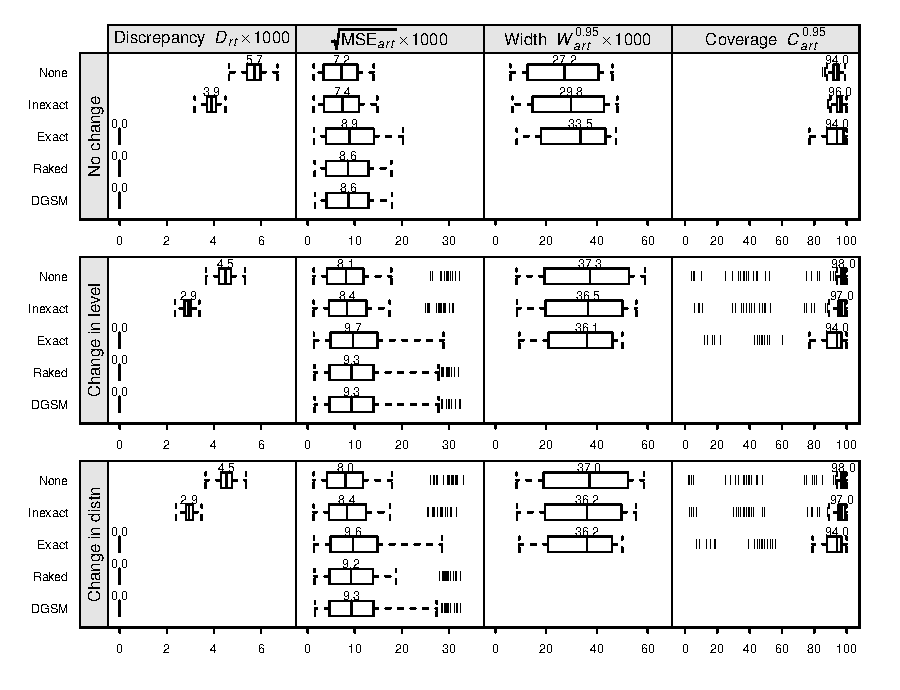
\includegraphics{out/fertility/fertility_performance_all}
    \caption{\small Performance of models of fertility rates, by type of benchmarking and dataset.}
    \label{fig:fertility_performance_all}
\end{figure}

The top row of Figure~\ref{fig:fertility_performance_all} gives results for the `no change' datasets, where the analysis model is correctly specified.  The model without benchmarking departs furthest from the benchmarks, but has the lowest MSE.  The version of our model with exact benchmarking has the opposite strengths and weaknesses, agreeing exactly with the benchmarks (by construction), but having the highest MSE.  The raked and DGSM estimators also obtain complete agreement, but with median MSE that is approximately 3-4\% lower than the model with exact benchmarking.  The model with inexact benchmarking is in an intermediate position, with moderate agreement and moderate MSE.

The models with no benchmarking, inexact benchmarking, and exact benchmarking have coverage rates close to the nominal 95\%, but the model without benchmarking achieves this with the narrowest credible intervals. As noted above, the raked and DGSM estimators do not have uncertainty measures and therefore do not have coverage rates.

\begin{figure}
   \centering
   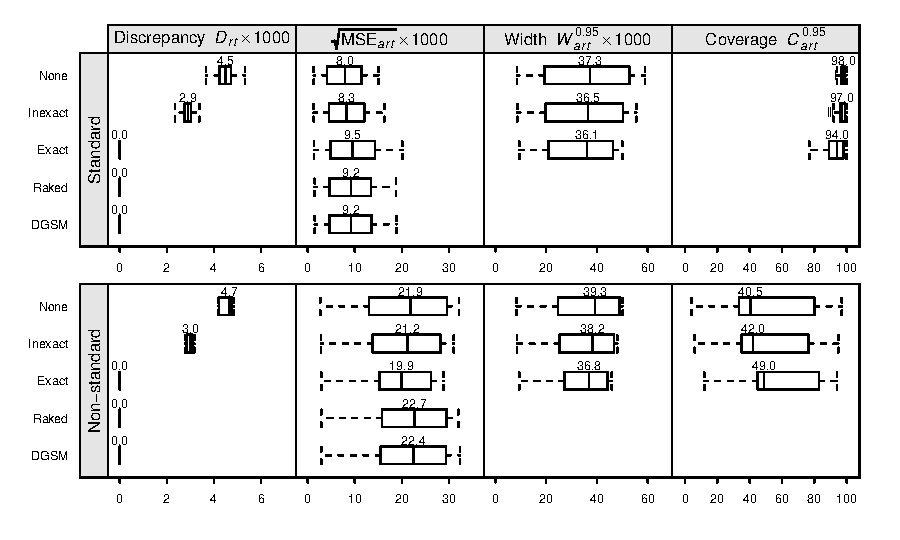
\includegraphics{out/fertility/fertility_performance_level}
   \caption{\small Performance of model of fertility rates when applied to `change in level' datasets, distinguishing between standard and nonstandard aras}.
   \label{fig:fertility_performance_level}
 \end{figure}

The second row of Figure~\ref{fig:fertility_performance_all} shows results for the `change in levels' datasets. The rank order of the discrepancy measures and MSEs is preserved.  The rank order of the width of credible intervals has changed, with the model without benchmarking having the widest credible intervals. In general, credible intervals are wider than in the `no change' case, but coverage rates for a subset of areas are poor, with and without benchmarks.  Similar results are obtained with the `change in distribution' datasets.

 \begin{figure}
   \centering
   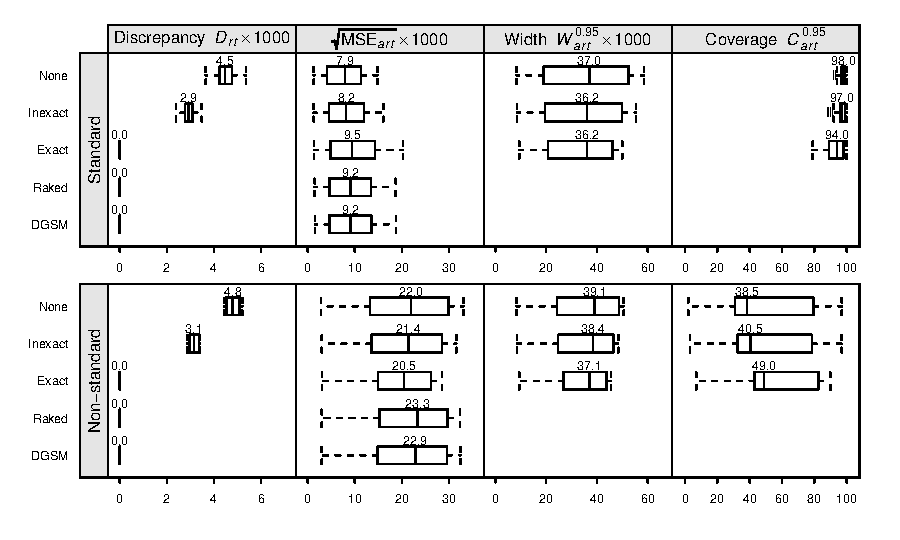
\includegraphics{out/fertility/fertility_performance_distn}
   \caption{\small Performance of model of fertility rates when applied to `change in distribution' datasets, distinguishing between standard and nonstandard areas.}
   \label{fig:fertility_performance_distn}
 \end{figure}

Figure~\ref{fig:fertility_performance_level} shows results for the `change in levels' datasets, but distinguishing between standard and non-standard areas.  In the standard areas, performance is similar to the overall picture in Figure~\ref{fig:fertility_performance_all}.  In the nonstandard areas, our benchmarked models have smaller MSE than the non-benchmarked model, and the raked and DGSM estimators. Coverage rates for the nonstandard areas are poor for all three versions of our model, but the model with exact benchmarking has better coverage rates than the other two.  As can be seen in Figure~\ref{fig:fertility_performance_distn}, a similar pattern is found with `change in distribution' datasets.

\subsection{Estimation of Smoking Prevalence from Survey Data}
  \label{sec:smoking}

In the second simulation we compare the performance of benchmarked and non-benchmarked models when estimating finite-population quantities.

Ideally, the distinction between finite-population and super-population quantities should be reflected in the benchmarking procedures, so that, for instance, agreement with $\bm{m}$ is measured using the finite-population equivalent of $\bm{\psi}$.  We have not done so, on pragmatic grounds.  Using super-population quantities simplifies the MCMC computations, and when sample sizes are large, as they typically are for aggregate quantities such as $\bm{m}$ and $\bm{\psi}$, super-population quantities closely approximate finite-population ones.

The simulation uses artificial surveys of smoking prevalence constructed from real data from the 2013 New Zealand population census.
The artificial surveys are generated by randomly drawing records from a file containing unit-level census data on the population aged 15 and over.  The file contains information on age, sex, region within the country, income level, and whether the respondent currently smokes.  The file excludes the 8 percent of people who did not answer the smoking question, leaving a total of 3.07 million records.  At each replicate of the simulation, we construct a simulated survey dataset by drawing a sample of 60,000 records from the file.  The sample is stratified by region, with simple random sampling within each region.  There are 16 regions in total, with populations ranging from 23,000 to just over 1 million.  Regional sample sizes are proportional to the square root of regional population size.

Let $N_{aslr}$ be the number of people in age-group $a \in$ \{15--24, 25--34, $\dots$, 55--64, 65+\}, sex $s$, income level $l \in$ \{No income or loss, \$1--\$20,000, \$20,001--\$40,000, \$40,001--\$60,000, \$60,001--\$100,000, \$100,001+\}, and region $r \in \{1, \dots, 16\}$.  Let $Y_{aslr}$ be the number of people who smoke. We treat the census file as the true finite population.  Within the simulated analysis, $N_{aslr}$ is known but $Y_{aslr}$ is not.    The aim of the simulated analysis is to estimate finite-population smoking prevalence by age, sex, and income, $p_{asl} = \sum_r Y_{aslr} / \sum_r N_{aslr}$.

Let $y_{aslr}$ and $n_{aslr}$ be the sample equivalents of $Y_{aslr}$ and $N_{aslr}$.  The model
\begin{align}
  y_{aslr}  & \ind \text{Binomial} \left( n_{aslr}, \gamma_{aslr} \right) \\
  \text{logit}(\gamma_{aslr}) & \ind \text{N}\left( \beta^0 + \beta_a^{\text{age}} + \beta_s^{\text{sex}} + \beta_l^{\text{income}} + \beta_r^{\text{reg}} + \beta_{al}^{\text{age:income}}, \sigma^2 \right)
\end{align}
is fitted to the artificial survey data.  Region is included in the model to account for the stratified sample design.  The age effects, income effects, region effects, and age-income interaction all have normal priors with mean 0.  However, following the approach that \citet{little2012calibrated} suggests for statistical agencies that are reluctant to adopt informative priors, we use improper uniform priors over the set of positive real numbers for the standard deviation terms. We use an improper uniform prior for the sex effect.

The model is fitted without benchmarking, and with exact and inexact benchmarking.  The benchmarks are estimated mean smoking prevalence by income level $$m_l = \frac{\sum_{a,s,r} N_{aslr}y_{aslr}/n_{aslr}}{\sum_{a,s,r} N_{aslr}}.$$  The corresponding super-population benchmarking parameters are $$\psi_l=\sum_{a,s,r}N_{aslr}\gamma_{aslr}/\sum_{a,s,r}N_{aslr}.$$ The finite-population equivalent of $\psi_l$ is $\psi_l^{\text{fin}}=\sum_{a,s,r}Y_{aslr}/\sum_{a,s,r}N_{aslr}$.

Under exact benchmarking, $p^{[\bm{m}|\bm{\psi}]}(\bm{m} | \bm{\psi})$ is given by \eqref{eq:model_exact_benchmarking}.  Under inexact benchmarking, $p^{[\bm{m}|\bm{\psi}]}(\bm{m} | \bm{\psi})$ is given by \eqref{eq:dist-normal}, which becomes
\begin{equation}
p^{[\bm{m}|\bm{\psi}]}(\bm{m}|\bm{\psi})\propto \text{exp}\left( -\sum_l \frac{ (m_l-\psi_l)^2}{ 2 \lambda s_l^2} \right), \label{eq:dist-normal-smoking}
\end{equation}
where $s_l$ is the standard error of using $m_l$ to estimate $\psi_l$. We examine the cases where $\lambda=1$ and where $\lambda=0.5$.

Benchmarks $m_l$ and standard errors $s_l$ are calculated using function \code{svymean} from \proglang{R} package \code{survey} \citep{lumley2004analysis}.  Calculating standard errors that properly account for the stratified sample design is complicated; function \code{svymean} uses replicate weights \citep[][p. 32]{lumley2011complex}.

Performance measures $D_l$, $\text{MSE}_{asl}$, $W_{asl}^q$, and $C_{asl}^q$ are calculated for finite-population smoking prevalence $p_{asl}$.
Here $D_l$ is defined as
\begin{equation}
  D_l =  \text{E}\left( \frac{ | \bar{\psi}_l^{\text{fin}} - m_l | }{ s_l }\right),  \label{eq:defn_agree2}
\end{equation}
where $\bar{\psi}_l^{\text{fin}}$ is the posterior mean of $\psi_l^{\text{fin}}$.  This measures discrepancies in units of standard errors.
To estimate $p_{asl}$ and $\psi_l^{\text{fin}}$, it is necessary to estimate $Y_{asl} = \sum_r (y_{aslr} + y_{aslr}^{\text{non}})$, where $y_{aslr}^{\text{non}}$ is the number of non-sampled people in area $aslr$ who smoke.  Draws from the posterior distribution of $y_{aslr}^{\text{non}}$ can be generated using $y_{aslr}^{\text{non} (t)} \sim \text{Binomial}(N_{aslr} - n_{aslr}, \gamma_{aslr}^{(t)})$, where $\gamma_{aslr}^{(t)}$ is the $t$th draw from the posterior sample for $\gamma_{aslr}$.

As with the fertility simulation, we use $K = 100$ replicates.  The Gibbs sampler is run with 6 independent chains, each with 100,000 iterations. Every 250th draw from the final 50,000 iterations of each chain is recorded, yielding a combined total of 1,200 draws from the posterior distribution.

\begin{figure}
  \center
    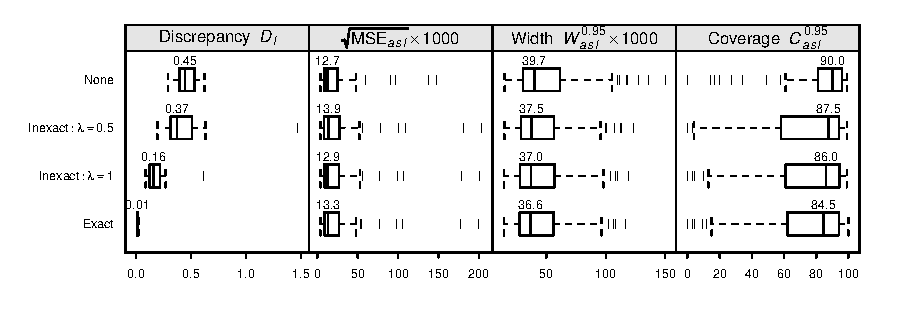
\includegraphics{smoking/smoking_performance}
  \caption{\small Performance of model of smoking prevalence, by type of benchmarking}
  \label{fig:smoking_performance}
\end{figure}

The results from the simulation are summarized in Figure~\ref{fig:smoking_performance}, with $q=0.95$.  Benchmarking improves agreement between the model-based estimates and the benchmarks, with exact benchmarking giving the largest improvement, and inexact benchmarking with $\lambda=1$ the smallest.  Exact benchmarking does not achieve complete agreement, since the benchmarks are applied to super-population prevalences, rather than finite population ones.  However, the median absolute difference between model-based estimates and benchmarks is only 0.01 standard errors.

Benchmarking degrades overall accuracy and coverage. However, the most striking feature of the distributions of $\text{MSE}_{asl}$, $W_{asl}^{0.95}$, and $C_{asl}^{0.95}$ in  Figure~\ref{fig:smoking_performance} is the long tails.  These long tails result from a small number of outliers, notably people aged 15--24 with incomes of \$100,000 or higher.  This group has high smoking prevalence, even though youth and high incomes are, in general, associated with low prevalence.  With these particular data, rather than providing robustness to outliers, benchmarking decreases robustness.

\section{Application}
  \label{sec:application}

We now apply fully Bayesian benchmarking to a real dataset.  We estimate age-sex-specific mortality rates for local authority districts in England and Wales, using as benchmarks sex-specific life expectancies for regions.  All code and data for the application can be obtained from [GitHub address].

Our data are counts of deaths and populations at risk in 2014, disaggregated into 20 age groups, 2 sexes, and 348 local authority districts. The total number of deaths is 500,314, and the total population at risk is 57,408,654.  The median number of deaths per area is 8, and 16\% of areas have 0 deaths.  Direct estimates of mortality rates (i.e., counts of deaths for each area, divided by the corresponding population at risk) for 5 randomly-selected districts are shown in Figure~\ref{fig:mx_examples}.  Because the graphs are drawn on a log scale, estimates for which the count of deaths and direct estimate are 0 are omitted.  As is apparent from the graphs, direct estimates of age-sex-specific mortality rates at the district level are unstable below age 60.

\begin{figure}
  \center
    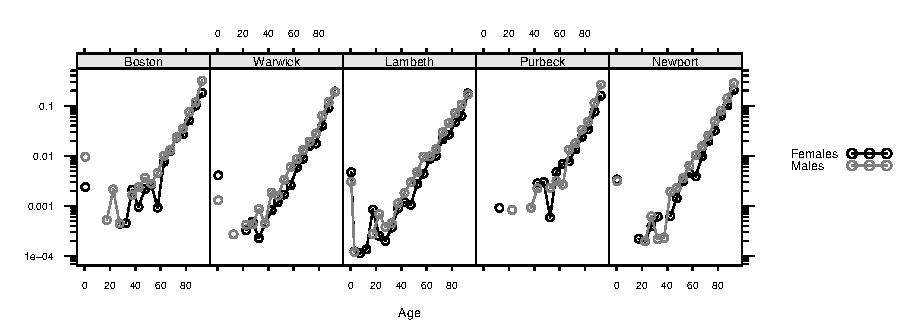
\includegraphics{out/mortality/mortality_mx_examples}
  \caption{\small Direct estimates of mortality rates, by age and sex, in 5 randomly-selected local authority districts in England and Wales, 2014. For some combinations of age, sex, and district, the counts of deaths, and hence direct estimates, are 0. Estimates for these combinations are not shown, since the graph is on a log scale. }
  \label{fig:mx_examples}
\end{figure}

Let $y_{asd}$ be the count of deaths for age group $a$, sex $s$ and district $d$, and let $\gamma_{asd}$ and $w_{asd}$ be the corresponding mortality rate and population at risk.  We apply the model
\begin{align}
  y_{asd} & \ind \text{Poisson}( w_{asd} \gamma_{asd} ) \\
  \log \gamma_{asd} & \ind \text{N} \left( \beta^0 + \beta_a^{\text{age}} + \beta_s^{\text{sex}} + \beta_d^{\text{dis}} + \beta_{as}^{\text{age:sex}}, \sigma^2 \right). \label{eq:log_gamma_mortality}
\end{align}
Age effects are assumed to follow a random walk with drift,
\begin{align}
  \beta_a^{\text{age}} & \sim t_4(\eta_a^{\text{age}}, \tau_{\text{age}}^2) \label{eq:mortality_age_prior_start} \\
  \eta_0^{\text{age}} & \sim \text{N}(0, 10^2) \\
  \eta_a^{\text{age}} & \sim \text{N}(\eta_{a-1}^{\text{age}} + \delta_{a-1}^{\text{age}}, \omega^2), \quad a > 0 \\
  \delta_0^{\text{age}} & \sim \text{N}(0, 1) \\
  \delta_a^{\text{age}} & \sim \text{N}(\delta_{a-1}^{\text{age}}, \varphi^2), \quad a > 0 \label{eq:mortality_age_prior_end}.
\end{align}
The drift term accounts for the fact that log-mortality rates rise linearly over much of the age range.
The use of a $t_4$ distribution in \eqref{eq:mortality_age_prior_start} allows for occasional large departures from trend, as occurs at age 0.  The sex effect has a normal prior $\beta_s^{\text{sex}} \sim \text{N}(0,1)$.  The district effect has a normal prior $\beta_d^{\text{dis}} \sim \text{N}(0, \tau_{\text{dis}}^2)$, with a weakly informative half-$t$ prior on the standard deviation, $\tau_{\text{dis}} \sim t_7^{+}(0, 1)$.  The interaction has a normal prior $\beta_{as}^{\text{age:sex}} \sim \text{N}(0, \tau_{\text{age:sex}}^2)$, with a weakly informative half-$t$ prior on the standard deviation, $\tau_{\text{age:sex}} \sim t_7^{+}(0, 0.5^2)$.  We use a smaller scale for the interaction than for the main effect on the principle that interactions are typically smaller in size than main effects \citep{gelman2008weakly}.  Standard deviations terms $\sigma$, $\tau_{\text{age}}$, $\omega$ and $\varphi$ all have $t_7^{+}(0, 1)$ priors.

We benchmark the estimates to sex-specific life expectancies for regions.  The region is an administrative unit further up the English geographical hierarchy than the local authority district.  Counting Wales as one region, there were 10 regions in England and Wales in 2014. Life expectancy is the mean number of years a newborn baby would live if prevailing mortality rates were to continue indefinitely.  The procedure for calculating life expectancy is given in \citet[][ch. 3]{preston2001demography}, but for our purposes, the key point is that life expectancy is a nonlinear deterministic function of age-specific mortality rates.

Let
\begin{equation}
  \zeta_{asr} = \sum_{d \in \Delta_r} w_{asd} \gamma_{asd} / \sum_{d \in \Delta_r} w_{asd} \label{eq:aggregate_mort_rates}
\end{equation}
be the mortality rate in age group $a$, sex $s$ and region $r$, where $\Delta_r$ is the set of $d$ such that district $d$ belongs to region $r$.  Life expectancy for sex $s$ in region $r$ is
\begin{equation}
  \psi_{sr} = f_{\text{life}}(\zeta_{1sr}, \cdots, \zeta_{Asr}), \label{eq:calc_life_exp}
\end{equation}
where $f_{\text{life}}$ is the nonlinear function for calculating life expectancy from age-specific mortality rates, and $A=20$ is the number of age groups.  Similarly, let
\begin{equation}
  z_{asr} = \sum_{d \in \Delta_r} y_{asd} / \sum_{d \in \Delta_r} w_{asd}
\end{equation}
be the direct estimate of the mortality rate in age group $a$, sex $s$, and region $r$.  The benchmark for sex $s$ and region $r$ is then
\begin{equation}
  m_{sr} = f_{\text{life}}(z_{1sr}, \cdots, z_{Asr}). \label{eq:calc_life_exp}
\end{equation}
Since life expectancies are ordinarily reported to at most two decimal places, most users can tolerate discrepancy of size 0.01.
We specify agreement with the benchmarks as
\begin{equation}
  m_{sr} \ind \text{N}(\psi_{sr}, 0.005^2).
\end{equation}

We fit our model with and without benchmarks, using 4 independent chains, each with 80,000 iterations.  Every 100th draw from the final 40,000 iterations of each chain is recorded, yielding a combined total of 1,600 draws from the posterior distribution.

Benchmarking improves agreement between the modelled life expectancies by sex and region and the benchmarks.  Figure~\ref{fig:mortality_life_exp_regions} compares benchmarks with point estimates (posterior medians) from models with and without benchmarking.  Without benchmarking, the model-based estimates are noticeably different from the benchmarks, especially for males.  With benchmarking, the model-based estimates and benchmarks are indistinguishable.

\begin{figure}
  \center
    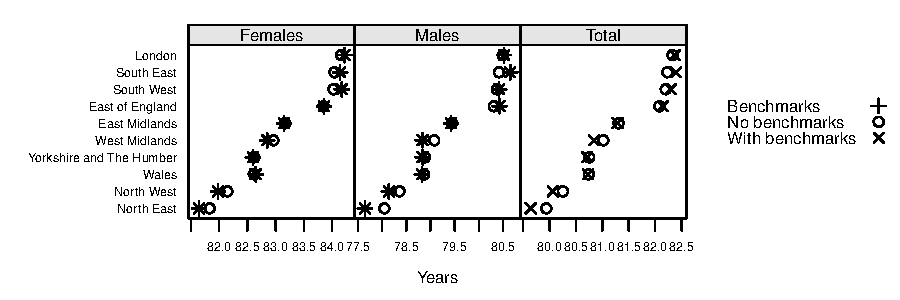
\includegraphics{out/mortality/mortality_life_exp_regions}
  \caption{\small Point estimates of life expectancy by sex and region: benchmarks versus posterior medians from models.}
  \label{fig:mortality_life_exp_regions}
\end{figure}

\begin{figure}
    \begin{subfigure}[b]{\textwidth}
     \center
    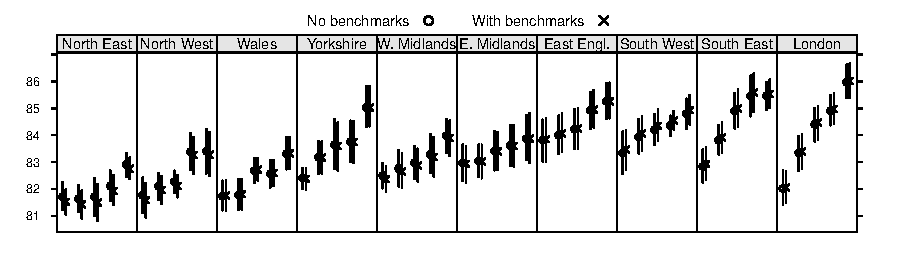
\includegraphics{out/mortality/mortality_lx_change_females}
      \caption{\small Females}
        \label{fig:mortality_lx_change_females}
    \end{subfigure}
    \begin{subfigure}[b]{\textwidth}
     \center
    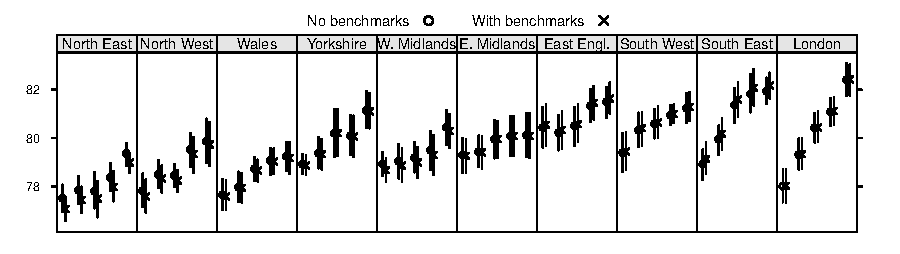
\includegraphics{out/mortality/mortality_lx_change_males}
      \caption{\small Males}
        \label{fig:mortality_lx_change_males}
    \end{subfigure}
  \caption{\small Life expectancies for 50 local authority districts, with 5 randomly-selected districts from each region.  The vertical lines are 95\% credible intervals.}
  \label{fig:mortality_lx_change}
\end{figure}

Figure~\ref{fig:mortality_lx_change} shows life expectancies by sex and district, with and without benchmarking.  Benchmarking shifts most posterior medians.  The shifts are larger in some regions, such as the North East, than in others, such as London.  Benchmarking changes the width of credible intervals, but only very slightly.  The mean width of credible intervals for all age-sex-district-specific log-mortality rates increases from 0.33 to 0.34, and the mean width of credible intervals for sex-district-specific life expectancies decreases from 1.33 to 1.32 (results not shown).

Figure~\ref{fig:mortality_mx_change} illustrates how benchmarking affects age-sex-specific mortality rates at the district level.  The percent differences between posterior medians of mortality rates from benchmarked models and those from non-benchmarked models are all below 10\%.

\begin{figure}
  \center
    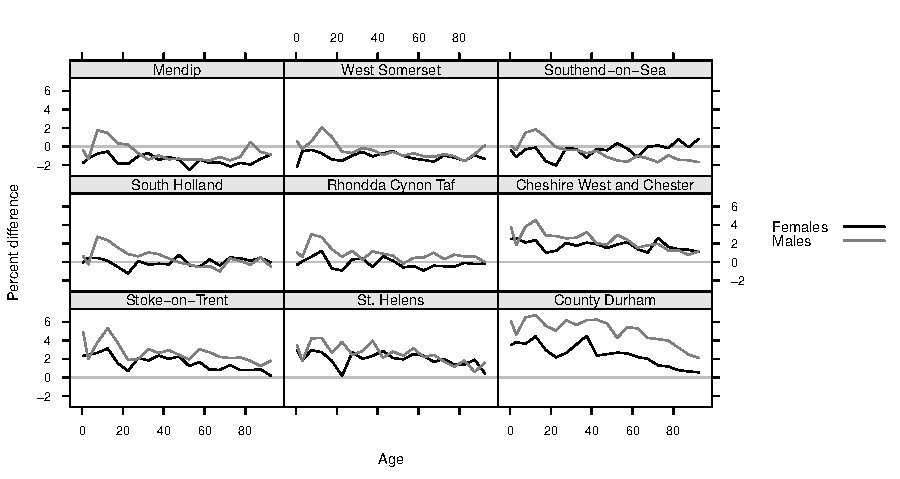
\includegraphics{out/mortality/mortality_mx_change}
  \caption{\small Percent differences between posterior medians from benchmarked models and posterior medians from non-benchmarked models, for age-sex-specific mortality rates in 9 randomly-selected local authority districts.}
  \label{fig:mortality_mx_change}
\end{figure}


\section{Discussion}
  \label{sec:discussion}
We conclude by summarizing the advantages of the benchmarking methods described in this paper.

In many applications of small area estimation, uncertainty can be large enough to affect decision making.  With the complicated models often used in
modern applications of small area estimation, deriving uncertainty measures can be difficult. Our approach to benchmarking allows full posterior distributions to be generated for a wide range of models, which can be used to produce uncertainty measures.

In some applications, the small area parameters are not the main focus of interest, but are instead inputs into other calculations. For instance, when comparing the performance of schools or hospitals, the absolute pass rates or recovery rates may be less important than the rankings. Our approach can be used to produce a full posterior distribution for rankings or other functions of the small area parameters, and to produce the associated uncertainty measures.

With some applications, it is not necessary to obtain complete agreement between benchmarks and model-based estimates. Policy analysts, for instance, may have weaker requirements for agreement among estimates than administrators. In such cases, inexact benchmarking, using the methods described in this paper, gives statisticians the ability to control the level of agreement with the benchmarks.

Finally, in some applications, the most natural benchmarks are quantities that have a non-linear relationship with the small area parameters, which can be accommodated under our approach. In this paper, we consider the case of life expectancies, but other non-linear benchmarks such as growth rates and ratios can also be implemented using our methods.


\bibliographystyle{apalike}
\bibliography{fbb}

\end{document}

